\section{Results}
\label{sec:resul}

All results were obtained in simulation, with the default sea of the simulator, which moves the winch up and down by about $0.25\,\text{m}$, without wind unless stated otherwise, and with the state of both vehicles taken from the simulator.

\begin{figure*}[t]
    \centering
    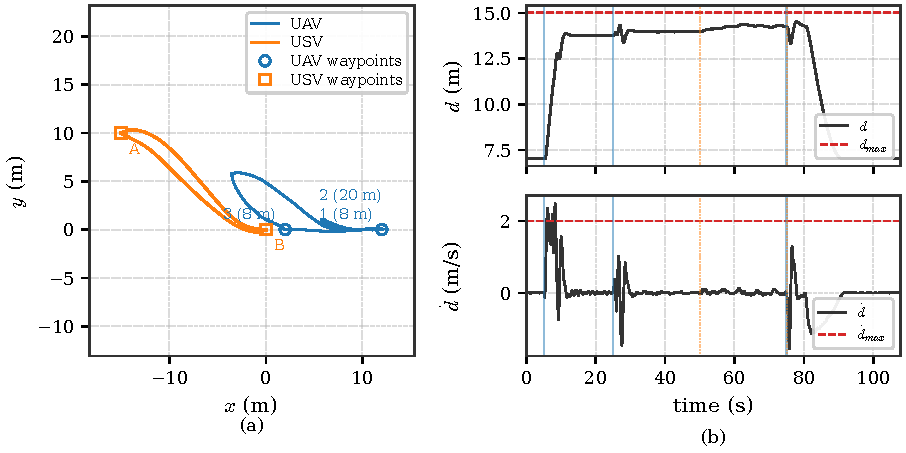
\includegraphics[width=0.8\textwidth]{Results/figures/01_tracking/steps_tether.pdf}
    \caption{Step references: (a) paths and waypoints, with the height of those of the UAV, and (b) separation $d$ and its rate $\dot d$, with their limits; vertical lines mark the steps of the UAV (solid) and of the USV (dotted).}
    \label{fig:steps}
\end{figure*}

\subsection{Tracking}

The tracking was first measured on a reference that both vehicles can follow. The USV sails a circle of $3\,\text{m}$ radius at $0.15\,\text{m/s}$, while the UAV flies a circle of $5\,\text{m}$ about the same centre at $1.5\,\text{m/s}$, tilted so that its height goes from $21$ to $29\,\text{m}$. Since the two circles are flown at different angular speeds, the separation varies between $20$ and $29\,\text{m}$, and so does the force of the tether, between $3.9$ and $6.0\,\text{N}$. For comparison, the same circle was also flown by the position controller of PX4, which receives the position, velocity and acceleration of the reference, is not aware of the tether, and compensates constant forces through the integral action of its velocity loop.


Figure~\ref{fig:nominal} and Table~\ref{tab:nominal} show that the NMPC follows the circle with less than half the error of PX4, $4.0$ against $9.0\,\text{cm}$. Neither keeps an offset in height, and the difference lies in the timing: PX4 reacts to the error once it has appeared, and follows the reference about $45\,\text{ms}$ behind it, while the NMPC anticipates its motion over the horizon. The USV follows its circle within $0.6\,\text{cm}$, and the two NMPCs take on average $4.8$ and $1.9\,\text{ms}$ of their sampling periods of $20$ and $100\,\text{ms}$.

\begin{table}[t]
    \centering
    \caption{Position error of the UAV on the tilted circle (cm), over $68\,\text{s}$.}
    \label{tab:nominal}
    \footnotesize
    \begin{tabular}{@{}lrrrrr@{}}
        \toprule
        Controller & RMSE & Max. & $x$ & $y$ & $z$ \\
        \midrule
        NMPC & $4.0$ & $5.3$ & $2.6$ & $2.5$ & $1.7$ \\
        PX4 & $9.0$ & $11.6$ & $5.9$ & $5.9$ & $3.2$ \\
        \bottomrule
    \end{tabular}
\end{table}

\begin{figure*}[t]
    \centering
    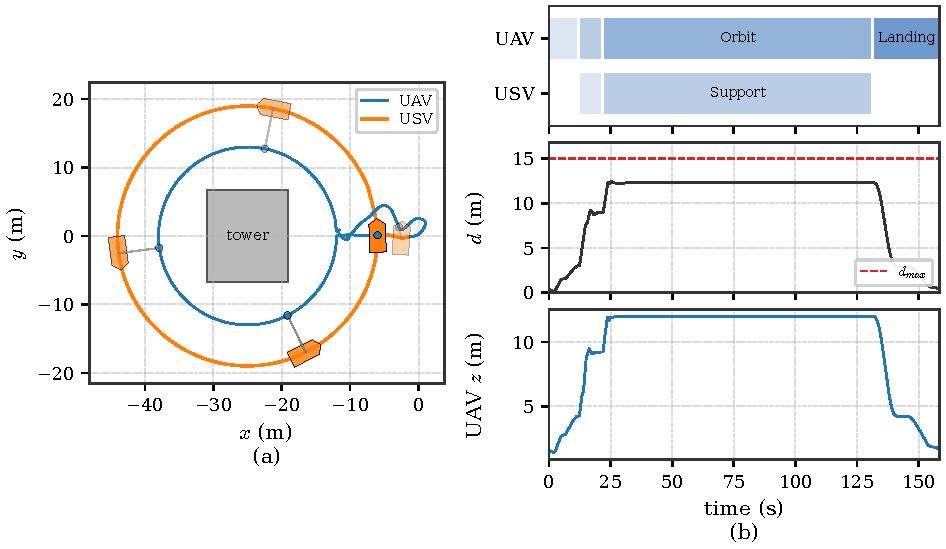
\includegraphics[width=0.85\textwidth]{Results/figures/02_missions/inspection.pdf}
    \caption{Inspection mission: (a) paths of both vehicles around the tower, with their positions and the tether at five instants, and (b) manoeuvres of each vehicle, separation $d$ and height of the UAV.}
    \label{fig:inspection}
\end{figure*}

\subsection{Planning}

To test the planning, both vehicles were given step references, single points held fixed over the horizon, with $d_{max} = 15\,\text{m}$. The UAV is sent $10\,\text{m}$ sideways, then $12\,\text{m}$ up, to a point $22\,\text{m}$ from the winch, beyond the reach of the tether; the USV is then sent $18\,\text{m}$ away, and both finally return, Figure~\ref{fig:steps}.


When its reference lies beyond the reach of the tether, the UAV stops short of it, on the line towards it, at $14\,\text{m}$ from the winch, and when the USV then sails away, it follows the USV, with the separation between $14.0$ and $14.4\,\text{m}$. In the first step, moving sideways at the same height would separate the vehicles faster than the winch pays out the tether, and the UAV drops by $2\,\text{m}$ on the way to slow the growth of the separation, whose rate exceeds its limit of $2\,\text{m/s}$ only briefly at the start of the step. The steps bring the actuators to their limits: the thrust of the UAV saturates at its maximum and its commanded tilt at $28.6^\circ$, while the thrusters of the USV reach their maximum reverse thrust and their maximum angle as it turns in place. The rates of all the commands reach their limits without exceeding them, and the real pitch of the UAV exceeds its limit by at most $1.7^\circ$, as the attitude loop of the autopilot slightly overshoots its command. The controllers therefore do not need feasible, or even continuous, references, which keeps the manoeuvres simple.


\begin{figure*}[t]
    \centering
    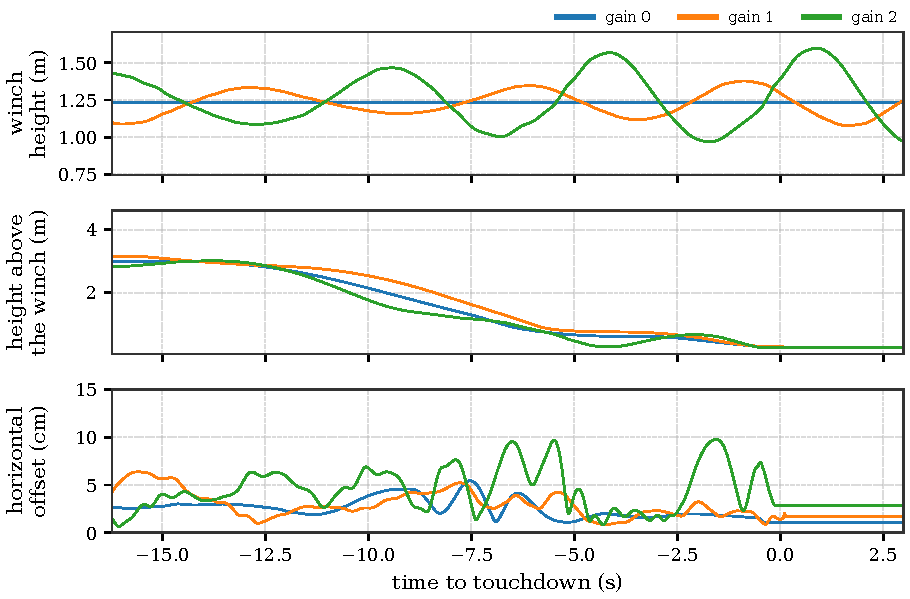
\includegraphics[width=0.7\textwidth]{Results/figures/03_disturbances/waves_landing.pdf}
    \caption{Landing with waves, from the start of the descent to the touchdown: height of the winch, height of the UAV above it, and horizontal offset from it.}
    \label{fig:waves}
\end{figure*}

\begin{figure*}[t]
    \centering
    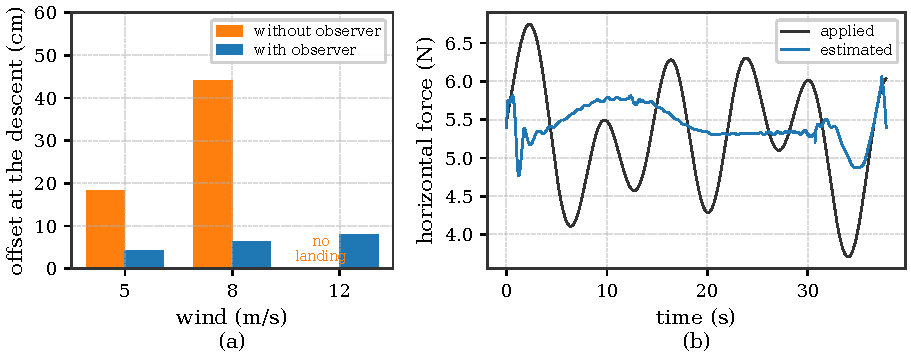
\includegraphics[width=0.8\textwidth]{Results/figures/03_disturbances/wind.pdf}
    \caption{Landing with wind: (a) offset of the UAV from the winch when the descent starts, and (b) force of a $12\,\text{m/s}$ wind and estimate of the observer.}
    \label{fig:wind}
\end{figure*}

\subsection{Missions}

The three missions were flown with $d_{max} = 15\,\text{m}$, and are summarised in Table~\ref{tab:missions}. In the scout, the UAV keeps $8\,\text{m}$ ahead of the bow of the USV as it sails a route with two turns of $90^\circ$, with a mean error of $5\,\text{cm}$, largest at the turns, where the point ahead of the bow swings around the USV. In the patrol, the UAV detects a fleeing target $19\,\text{m}$ away, beyond the reach of the tether; its reference is brought within reach along the line from the USV, which lowers it, and the UAV is above the target $5\,\text{s}$ after the detection, while the USV, at up to $2.2\,\text{m/s}$, catches up with it $21\,\text{s}$ after the detection.


The inspection, Figure~\ref{fig:inspection}, shows best how the two vehicles work as one system. The UAV circles a tower of $12$ by $13\,\text{m}$ at a radius of $13\,\text{m}$, a circle beyond the reach of the tether from any fixed point. Its reference is a circle fixed in the world, regardless of the USV, while the USV supports it from the water, $6\,\text{m}$ further from the tower. The USV keeps within $3\,\text{cm}$ of its intended radius around the whole tower, the separation stays at $12.3\,\text{m}$, and the UAV follows its circle within $1\,\text{cm}$, so that the two vehicles together cover a circle that neither could cover alone.

\begin{table}[t]
    \centering
    \caption{Missions with $d_{max} = 15\,\text{m}$: duration, largest separation, and distance of the touchdown from the centre of the pad.}
    \label{tab:missions}
    \footnotesize
    \begin{tabular}{@{}lrrr@{}}
        \toprule
        Mission & Duration & Max. $d$ & Touchdown \\
        \midrule
        Scout & $132\,\text{s}$ & $9.6\,\text{m}$ & $3\,\text{cm}$ \\
        Inspection & $159\,\text{s}$ & $12.5\,\text{m}$ & $4\,\text{cm}$ \\
        Patrol & $104\,\text{s}$ & $14.7\,\text{m}$ & $5\,\text{cm}$ \\
        \bottomrule
    \end{tabular}
\end{table}

\subsection{Waves and Wind}

The disturbances were added during the landing on the deck of the USV, sailing a route at $0.75\,\text{m/s}$. With the gain of the wave field raised to $1$ and $2$, the winch rises and falls by $0.25$ and $0.44\,\text{m}$, Figure~\ref{fig:waves}. The landing takes the same $25$ to $27\,\text{s}$ in all sea states, since the reference is taken above the mean height of the winch, and the UAV touches down $0$, $2$ and $4\,\text{cm}$ from the centre of the pad. What the waves change is the contact: the final approach aims below the deck, so the speed of the contact is set by its motion, and grows from $0.15$ to $0.26$ and $0.39\,\text{m/s}$.


The wind was applied as a drag force on the UAV, with means of $0.9$, $2.4$ and $5.3\,\text{N}$ for $5$, $8$ and $12\,\text{m/s}$ and gusts of $\pm 30\,\%$, with and without the disturbance observer, Figure~\ref{fig:wind}. Without the observer, the UAV settles away from its reference, $18$, $44$ and $83\,\text{cm}$ from the centre of the pad before the descent, the landing waits for a centring that never happens, and at $12\,\text{m/s}$ the mission failed in both runs, once at the takeoff and once when the UAV, landing $0.8\,\text{m}$ off the centre, was blown off the edge of the pad. With the observer, whose estimate follows the force of the wind about $0.7\,\text{s}$ behind it, gusts included, the offset is $4$, $6$ and $19\,\text{cm}$ and the UAV lands within $8\,\text{cm}$ of the centre. The most exposed moment is then the takeoff, when a strong crosswind can tip the UAV against the pad while the winch still holds it, before the controller has any effect; the NMPC recovers it once it is released, after a drift of $5.5\,\text{m}$.

